\documentclass[12pt,letterpaper]{article}
\usepackage[latin1]{inputenc}
\usepackage[spanish]{babel}
\usepackage{amsmath}
\usepackage{amsfonts}
\usepackage{amssymb}
\usepackage[pdftex]{graphicx}
\usepackage{bm}


\usepackage{tikz}
\usetikzlibrary{calc, arrows, positioning,decorations.pathreplacing,shapes, arrows.meta}
\usepackage{pgfplots}
\pgfplotsset{compat=1.5.1}
\pgfplotsset{width=7cm,compat=1.8}
\usepackage{xcolor}
\usepackage{ifthen}
\newcommand*{\val}{100}


\usepackage[inline]{asymptote}

\DeclareGraphicsRule{.1}{mps}{*}{} 
\DeclareGraphicsRule{.2}{mps}{*}{}
\usepackage{lmodern}
%\usepackage{float}
\usepackage[left=4cm,right=3cm,top=3cm,bottom=3cm]{geometry}
\author{Juan David Arg�ello Plata}
\title{Dise�o y construcci�n de un sistema de producci�n de extractos vegetales}
%\usepackage{hyperref}
\setcounter{tocdepth}{5}
\setcounter{secnumdepth}{5}
% For dummy lipsum text
\usepackage{lipsum}
\usepackage{array}
\usepackage{ragged2e}
\usepackage{multirow}
\usepackage{adjustbox}
\bibliographystyle{IEEEtran}
%\usepackage[backend=biber]{biblatex}
%\usepackage{adjustbox}
\usepackage{gensymb}
\usepackage{pgfgantt}
\usepackage{rotating}
\usepackage{pdflscape}
\usepackage{tikz}
\usepackage{pgfplots}
\usepackage{floatrow}
%\usepackage[firstpage]{draftwatermark}
\usepackage{caption}
\usepackage{subcaption}
\usepackage{hyperref}
\hypersetup{
	colorlinks=false,
	linkbordercolor = {white}
}
%\SetWatermarkText{\includegraphics[scale=1.25]{Images/uis.png}}
% Table float box with bottom caption, box width adjusted to content
\makeatletter
\newfloatcommand{capbtabbox}{table}[][\FBwidth]

\renewcommand\paragraph{\@startsection{paragraph}{4}{\z@}%
            {-2.5ex\@plus -1ex \@minus -.25ex}%
            {1.25ex \@plus .25ex}%
            {\normalfont\normalsize\bfseries}}
\makeatother
\setcounter{secnumdepth}{4} % how many sectioning levels to assign numbers to
\setcounter{tocdepth}{4}    % how many sectioning levels to show in ToC

\usepackage{fancyhdr}
\pagestyle{fancy}


\begin{document}
\begin{titlepage}
	\centering
	\textbf{\textsc{{\Huge Proyecto 3: "Biof\'abrica prototipada de procesos de extracci\'on y bioproductos para industrias av\'icola, cosm\'etica y de alimentos" \hspace{0.25cm} PA 253 - Informe III - Etapa III}}}\\
	\vspace{3.25 cm}
	Autor\\
	\textbf{\textsc{{\Large Juan David Arg�ello Plata}}}\\
	Ingeniero Mec�nico\\
	\vspace{3.25 cm}
	Revisado por\\
	\vspace{0.25 cm}
	\textbf{\textsc{\Large Jairo Ren� Mart�nez Morales}}\\
	Qu�mico PhD.\\
	
	\vspace{3.25 cm}
	
	\textbf{\textsc{\Large Universidad Industrial de Santander}}\\
	\large Facultado de Ingenier�as F�sicomecanicas\\ Escuela de Ingenier�a Mec�nica\\ Maestr�a en Ingenier�a Mec�nica\\ 
	2020

\end{titlepage}
\tableofcontents
\listoffigures
\setcounter{secnumdepth}{0}
\begin{center}
	\section{Introducci\'on}
\end{center}

\noindent
\justify

En el presente documento se presentan los resultados del estudio din\'amico realizado al sistema de molienda, evaluando y optimizando par\'ametros como: energ\'ia de impacto, distribuci\'on de energ\'ia de impacto por tipo de bola y velocidad de las bolas antes del impacto empleando como par\'ametros de entrada la geometr\'ia de las aletas, el tama\~no de las bolas y la velocidad de rotaci\'on del molino.
\setcounter{secnumdepth}{4}
\begin{center}
	\section{Sistema de molienda}
\end{center}

\noindent
\justify

Durante la etapa de dise\~no funcional del molino de bolas, se definieron las siguientes dimensiones y par\'ametros operacionales:

\begin{itemize}
	\item Volumen de $0.633 \left[m ^3 \right]$.
	\item Di\'ametro de $0.813 [m]$.
	\item Longitud de $1.22 [m]$.
	\item Velocidad de rotaci\'on de $37.5 [rpm]$.
	\item Potencia m\'inima de operaci\'on $3.36 [hp]$.
\end{itemize}

\vspace{-1mm}

\noindent
\justify

Se realiz\'o una evaluaci\'on num\'erica para determinar la mejor configuraci\'on de las aletas del molino y tama\~nos de bola (ver Figura \ref{aletas}) que garantizan la mayor efectividad posible, a trav\'es de la evaluaci\'on de la \textit{energ\'ia de impacto} de las bolas y su \textit{distribuci\'on} sobre el molino. Para ello, se desarrollar\'o una simulaci\'on num\'erica, empleando el m\'etodo\footnote{Los m\'etodos num\'ericos son teoremas matem\'aticos que permiten describir la naturaleza de diferentes fen\'omenos de car\'acter f\'isico-qu\'imico. Son ampliamente usados en ingenier\'ia como metodolog\'ias predictivas durante el proceso de dise\~no funcional y mec\'anico.} de elementos discretos (DEM), validada mediante una metodolog\'ia te\'orica simplificada.

\begin{figure}[h!]
\centering
\begin{tikzpicture}
	%Molino
	\draw (0,0) circle (3.1cm);
	\draw[dashed, blue!50] (0,-4) -- (0,-2.5);
	\draw[dashed, blue!50] (0,0) -- (0,4);
	\draw[dashed, blue!50] (-4,0) -- (0,0);
	\draw[dashed, blue!50] (2.5,0) -- (4,0);
	\draw (-0.51,2.945) arc(-260:-190:3);
	\draw[red] (-0.51,2.945) -- (0,2.5) -- (0.51,2.945);
	\draw[red] (-2.945,0.51) -- (-2.5,0) -- (-2.945, -0.51);
	\draw (-2.945, -0.51) arc(-170:-100:3);
	\draw[red] (-0.51,-2.945) -- (0,-2.5) -- (0.51,-2.945);
	\draw (0.51, -2.945) arc(-80:-10:3);
	\draw[red] (2.945,0.51) -- (2.5,0) -- (2.945, -0.51);
	\draw (2.945,0.51) arc(10:80:3);
	
	\draw[blue!50!red, arrows={-Triangle[angle=90:5pt,blue!50!red,fill=blue!50!red]}] (3.4,0.8) arc(20:60:4.5) node [midway, above=2.6mm, right=0.2mm] {$\overrightarrow{T}$};
	
	%División volumétrica
	\draw[dashed, step=0.5cm, blue!60!green, pattern=north west lines, pattern color=blue!60!green] (-2.05,-2.05) -- (2.05,2.05) arc(45:12:3) -- (2.4, 0) -- (2.85,-0.55) arc(-12:-78:3) -- (0,-2.4) -- (-0.55,-2.85) arc(-102:-135:3) -- cycle;
	
	%Bolas
	\draw[dashed] plot [smooth] coordinates { (2.05,2.05) (1,2) (-1,1) (-2,-0.8) (-2.05,-2.05) };
	\draw[fill=blue!70!black] (-1,1) circle (1.2mm);
	\draw[blue!70!black, arrows={-Triangle[angle=90:3pt,blue!70!black,fill=blue!70!black]}] (-1,1) -- (-1,0.5) node [black, text width=0.5cm, below=0mm] {$m_2 \overrightarrow{g}$};
	\draw[fill=red!40!blue] (-2,-0.8) circle (1.5mm);
	\draw[red!40!blue, arrows={-Triangle[angle=90:3pt,red!40!blue,fill=red!40!blue]}] (-2,-0.8) -- (-2,-1.2) node [black, text width=0.5cm, below=-2mm] {$m_3 \overrightarrow{g}$};
	\draw[fill=green!50!red] (1,2) circle (0.8mm);
	\draw[green!50!red, arrows={-Triangle[angle=90:3pt,green!50!red,fill=green!50!red]}] (1,2) -- (1,1.6) node [black, text width=0.5cm, below=-2mm] {$m_1 \overrightarrow{g}$};
\end{tikzpicture}
\caption{Din\'amica interna del molino.}
\label{aletas}
\end{figure}

\subsection{An\'alsis cinem\'atico} \label{cinema}

\noindent
\justify

La trayectoria de las bolas es uno de los par\'ametros que determina la eficiencia del proceso de trituraci\'on, debido a la magnitud de la fuerza y posici\'on del impacto. Este se trata de un an\'alisis simplificado, se desprecia el di\'ametro y el coeficiente de fricci\'on de las bolas, entre otros par\'ametros, como se aprecia en la Figura \ref{simplify}.

\begin{figure}[h!]
\centering
\begin{tikzpicture}	
	\draw (0,0) circle (3cm);
	\draw[arrows={-Triangle[angle=90:2.5pt,black,fill=black]}] (2.1, 2.1) -- (1.5,2.8) node[text width=1mm, above] {$\overrightarrow{V_0}$};	
	\draw[arrows={-Triangle[angle=90:2.5pt,black,fill=black]}] (2.1,2.1) -- (1,2.1) node[text width=1mm, left=3mm] {$V_{0x}$};
	\draw[arrows={-Triangle[angle=90:2.5pt,black,fill=black]}] (2.1,2.1) -- (2.1,2.5) node[text width=1mm, above] {$V_{0y}$};
	\node at (1.6, 2.3) {$\phi$};
	
	%Nomenclatura
	\draw[arrows={-Triangle[angle=90:2.5pt,black,fill=black]}] (0,0) -- (0,1) node[above] {$y$};
	\draw[arrows={-Triangle[angle=90:2.5pt,black,fill=black]}] (0,0) -- (-1,0) node[above] {$x$}; 
	\draw[arrows={-Triangle[angle=90:2.5pt,black,fill=black]}] (3.4,1) -- (3.4,0) node[below] {$\overrightarrow{g}$}; 
	
	
	
	\draw[fill=blue] (2.05,2.05) circle (1mm);
	%\draw[dotted, green!50!red] (2.1, 2.1) -- (-2.1, -2.1);
	\draw[dashed] plot [smooth] coordinates { ( 2.1,2.1) (1.5,1.9) (0, 1) (-1.5,-1.4) (-2,-2) };
	\draw[dotted, blue] (-2.05,-2.05) circle (1mm);
	\draw[red!40!yellow, arrows={-Triangle[angle=90:5pt,red!40!yellow,fill=red!40!yellow]}] (0,3.4) arc(90:120:4.5) node [midway, above] {$\overrightarrow{\omega}$};
	
	\draw[arrows={-Triangle[angle=90:4pt,black,fill=black]}] (0,0) -- (2,2) node[text width=1mm, below] {$\vec{r_0}$};
	
	
\end{tikzpicture}
\caption{Cinem\'atica de una bola (an\'alisis simplificado).}
\label{simplify}
\end{figure}

\noindent
\justify

De la Figura \ref{simplify}, $\vec{V_0}$ es la velocidad inicial, $\phi$ es el \'angulo en el que se distribuye el material a triturar durante el funcionamiento del molino, $\omega$ es la velocidad angular, $\vec{r_0}$ es el vector posici\'on inicial y $\vec{g}$ es el vector aceleraci\'on de la gravedad.

\noindent
\justify

Sabiendo que el valor de la aceleraci\'on en la componente vertical $a_y$ es la gravedad y asumiendo que la aceleraci\'on horizontal tiene un valor constante, e igual a cero $\left( a_x = 0 \right)$, se tiene lo siguiente:

\begin{equation}
\vec{a} = -g \hat{j}
\end{equation}

\noindent
\justify

Sabiendo que la aceleraci\'on es la variaci\'on de la velocidad con respecto al tiempo, se tiene que:

\begin{equation}
\vec{V} = V_{0x} \hat{i} + \left(V_{0y} - gt \right) \hat{j}
\end{equation}

\noindent
\justify

De igual manera, siendo la velocidad la variaci\'on de la posici\'on con respecto al tiempo:

\begin{equation}
\vec{r} = \left(-x_0 + V_{0x} t \right) \hat{i} + \left(y_0 + V_{0y}t - \frac{g t^2}{2} \right) \hat{j}
\end{equation}

\noindent
\justify

La velocidad angular $\omega$ tiene un valor de $3.93 \left(rev /s \right)$ y el radio del molino $r$ es de $0.4065 [m]$, de modo que el valor de la velocidad inicial es de $1.6 [m/s]$. Para una trituraci\'on \'optima, se requiere que el \'angulo de distribuci\'on sea de $45 \degree$, de modo que:

\begin{equation*}
V_{0x} = V_0 \cos \phi \rightarrow V_{0x} = 1.13 [m/s]
\end{equation*}

\begin{equation*}
V_{0y} = V_0 \sin \phi \rightarrow V_{0y} = 1.13 [m/s]
\end{equation*}

\begin{equation}
\vec{V_0} = 1.13 \hat{i} + 1.13 \hat{j} [m/s]
\label{velocidad}
\end{equation}

\noindent
\justify

De igual manera, el vector posici\'on inicial queda de la siguiente forma:

\begin{equation*}
x_{0} = r_0 \cos \phi \rightarrow x_{0} = 0.29 [m]
\end{equation*}

\begin{equation*}
y_{0} = r_0 \sin \phi \rightarrow y_{0} = 0.29 [m]
\end{equation*}

\begin{equation}
\vec{r_0} = 0.29 \hat{i} + 0.29 \hat{j} [m]
\label{posicion}
\end{equation}

\noindent
\justify

Para definir la trayectoria del material dentro del molino, es necesario conocer el tiempo que tarda en realizar su recorrido. Para conocer el tiempo, se debe conocer la posici\'on en donde cae.

\begin{figure}[h!]
\centering
\begin{tikzpicture}
	\draw[arrows={-Triangle[angle=90:4pt,black,fill=black]}] (0,-3) -- (0,3) node[left] {$y$};
	\draw[arrows={-Triangle[angle=90:4pt,black,fill=black]}]  (-3,0) -- (3,0) node[below] {$x$};
	\draw[fill=blue] (2.1,-2.1) circle (0.5mm);
	\draw[fill=blue] (-2.1,2.1) circle (0.5mm);
	
	\draw[dashed, blue!60] (-2.05,2.05) -- (2.05,-2.05) arc(-45:-78:3) -- (0,-2.4) -- (-0.55,-2.85) arc(-102:-168:3) -- (-2.4,0) -- (-2.85,0.55) arc(-192:-225:3) -- cycle;
	\node[below=3mm] at (2.1,-2.1) {$\left(x_f, y_f \right)$};
	\node[above=1mm] at (-2.1,2.1) {$\left(x_0, y_0 \right)$};
	
	\draw[<-] (-1,0) arc(180:135:1);	
	\node[left] at (-1,0.5) {$\phi$};
\end{tikzpicture}
\caption{Tendencia de distribuci\'on del material.}
\label{dist}
\end{figure}

\noindent
\justify

De la Figura \ref{dist}, la distribuci\'on del material est\'a dada por la siguiente relaci\'on matem\'atica:

\begin{equation}
y \left(t_f \right) = -\tan \phi \, x_f \, t_f
\label{tiempo}
\end{equation}

\noindent
\justify

Relacionando las Ecuaciones \ref{posicion} y \ref{tiempo}, se obtiene:

\begin{equation}
t_f ^2 - \frac{2 \left(V_{0y} + V_{0x} \tan \phi \right)}{g} t_f - \frac{2}{g} \left( y_0 - x_0 \tan \phi \right) = 0
\label{tf}
\end{equation}

\noindent
\justify

Relacionando las Ecuaciones \ref{velocidad}, \ref{posicion} y \ref{tf} $t_f$ toma valores de $-0.14 [s]$ y $0.43 [s]$; de modo que una bola llega al punto de impacto en \textbf{\boldsymbol{$0.43 [s]$}}. La relaci\'on entre la posici\'on vertical $y$ con respecto a la posici\'on horizontal $x$ se puede apreciar en la Ecuaci\'on \ref{yx}.

\begin{equation}
y (x) = r \sin \phi + \left(r + \frac{x}{\cos \phi} \right) \sin \phi - \frac{g \left(r + \frac{x}{\cos \phi} \right) ^2}{2 \omega ^2 r^2}
\label{yx}
\end{equation}

\noindent
\justify

La posici\'on de una bola durante la etapa de molienda se puede observar en la Figura \ref{yxgraph}.

\begin{figure}[h!]
\centering
\begin{tikzpicture}
	\begin{axis}[grid = both, minor tick num=2,
			title = \textbf{Trayectoria de una bola},
			xlabel = {$x [m]$},
			ylabel = {$y [m]$}]
	\addplot file {xy.txt};
	\end{axis}
\end{tikzpicture}
\caption{Trayectoria de una bola sobre el molino.}
\label{yxgraph}
\end{figure}

\newpage

\subsection{Impacto}

\noindent
\justify

La frecuencia de impacto de las bolas est\'a definido por la Ecuaci\'on \ref{impacto}.

\begin{equation}
f_i = N_{bi} RPS \, \, \, f_i \in N
\label{impacto}
\end{equation}

\noindent
\justify

D\'onde $N_{bi}$ es el n\'umero de bolas, del tipo de bola $i$ que hay en el molino y $RPS$ es el n\'umero de revoluciones por segundo del molino. La frecuencia de impacto debe ser un n\'umero natural.

\noindent
\justify

Las distribuciones de la energ\'ia de impacto por bola se calcula de acuerdo a lo planteado en la Ecuaci\'on \ref{dist}.

\begin{equation}
Dist_i = \left( \frac{I_i}{\sum _{j=1} ^{N_{tb}} I_j} \right) *100
\label{dist}
\end{equation}

\noindent
\justify

D\'onde $Dist_i$ corresponde a la distribuci\'on de la energ\'ia de impacto del tipo de bola $i$ sobre el molino e $I_i$ a la energ\'ia de impacto de todas las bolas de tipo $i$.




\begin{center}
	\section{\textit{M\'etodo de elementos discretos} - DEM}
\end{center}

\noindent
\justify

El m\'etodo de elementos discretos (DEM) es un m\'etodo que modela fuerzas interpart\'icula basadas en par\'ametros de elasticidad y la superposici\'on de part\'iculas no deformadas, que se entiende como la cantidad de deformaci\'on necesaria para que puedan, f\'isicamente, ocupar el espacio en su actual configuraci\'on. Requiere de seis grados de libertad en cuerpos r\'igidos: tres en dos dimensiones y seis en tres dimensiones.

\begin{figure}[h!]
	\centering
	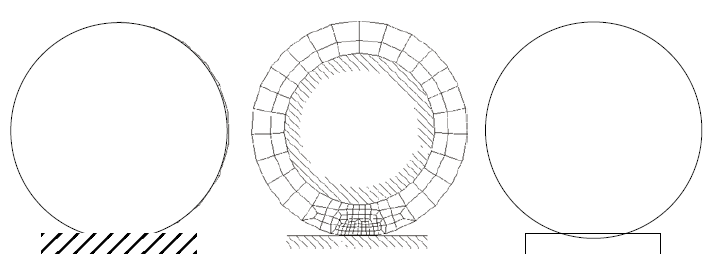
\includegraphics[width=\textwidth]{Images/DEM.PNG}
	\label{dem}
	\caption{Comparaci\'on entre metodolog\'ias de an\'alisis de part\'iculas para una esfera suave deformada en un plano: situaci\'on f\'isica real (izquierda), modelo analizado con el m\'etodo de elementos finitos (centro) y modelo con el m\'etodo de elementos discretos (derecha)}
\end{figure}

\noindent
\justify

El principio de este m\'etodo es el de computar las fuerzas proporcionales a la superposici\'on geom\'etrica de las part\'iculas empleadas. Para part\'iculas esf\'ericas, o circulares, las fuerzas involucradas son de tipo central; a diferencia de otras configuraciones geom\'etricas, debido a que deben caracterizar las fuerzas en la forma `d\'ebil' y `fuerte'. 

\noindent
\justify

Una simulaci\'on que emplea este m\'etodo num\'erico, normalmente se rige bajo los siguientes pasos:

\begin{enumerate}
	\item Detecci\'on de colisi\'on entre part\'iculas.
	\item Creaci\'on de una nueva interacci\'on y determinaci\'on de diferentes propiedades, entre ellas la rigidez.
\end{enumerate}

\noindent
\justify

Para interacciones ya existentes:

\begin{enumerate}
	\item Evaluaci\'on de deformaci\'on.
	\item Computaci\'on del esfuerzo basada en la deformaci\'on.
	\item Aplicaci\'on de fuerzas en la interacci\'on entre part\'iculas.
\end{enumerate}

\subsection{Detecci\'on de una colici\'on}

\noindent
\justify

La detecci\'on \textit{exacta} de colisi\'on entre dos part\'iculas requiere de un alto costo computacional. Tomando una pareja de cuerpos $i$ y $j$ y su colisici\'on `exacta' (en el sentido de precisi\'on admisible por la implementaci\'on num\'erica) presentadas en los puntos $P_i$ y $P_j$ la detecci\'on procede en los siguientes dos puntos:

\begin{enumerate}
	\item Detecci\'on de colisi\'on r\'apida usando puntos aproximados $\widetilde{P}_i$ y $\widetilde{P}_j$; siendo estos preconstrucciones en el modo que caracter\'isticas individuales $P_i$ y $P_j$ satisfacen la siguiente condici\'on mostrada en la Ecuaci\'on \ref{cond}.
	\begin{equation}
		\forall x \in R^3 : x \in P_i \rightarrow x \in \widetilde{P}_i
		\label{cond}
	\end{equation}
	De igual manera para $P_j$. El predicado aproximaado se conoce como `volumen l\'imite', siguiendo lo siguiente:
	\begin{equation}
		\left(\widetilde{P}_i \cap \widetilde{P}_j \right) = {\O} \rightarrow \left( P_i \cap P_j \right) = {\O}
		\label{imposible}
	\end{equation}
	\item Al filtrar las colisiones imposibles mediante la Ecuaci\'on \ref{imposible}, algoritmos de detecci\'on de mayor costo computacional pueden ser impementados al filtrar falsas parejas de colisi\'on restantes, como se observa en la Figura \ref{colision}.
	\begin{equation}
		\left(\widetilde{P}_i \cap \widetilde{P}_j \right) \neq {\O} \wedge \left(P_i \cap P_j \right) = {\O}
	\end{equation}
\end{enumerate}

\begin{figure}[h!]
\centering
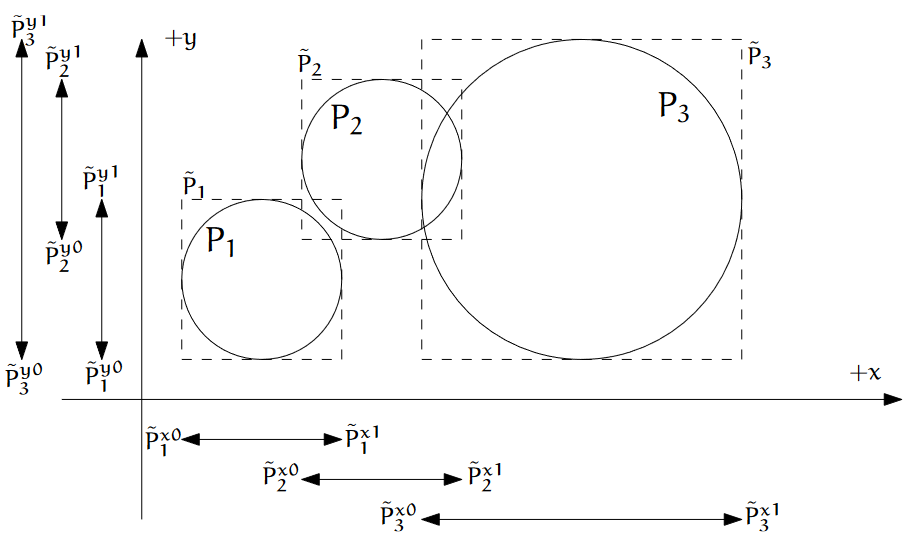
\includegraphics[width=0.85\textwidth]{Images/Colision.PNG}
\caption{Detecci\'on de colisi\'on entre part\'iculas.}
\label{colision}
\end{figure}
\newpage

\begin{center}
	\section{Simulaci\'on num\'erica}
\end{center}

\noindent
\justify

El material seleccionado, tanto para el molino como las bolas, es acero es acero A36. Las propiedades del mateial, empleadas para el desarrollo de la simulaci\'on num\'erica, se pueden apreciar en el Cuadro \ref{data}.

\begin{table}[h!]
\centering
\begin{tabular}{c c}
\hline
\textbf{Par\'ametro} &  \textbf{Valor} \\ \hline
Coeficiente de Posisson $(\nu )$ & $0.27$ \\ \hline
Densidad $(\rho )$ & $7850 \left[kg/m^3 \right]$ \\ \hline
M\'odulo de Young $(E )$ & $250 [MPa]$ \\ \hline
Coeficiente de restituci\'on & $0.9$ \\ \hline
Coeficiente de fricci\'on est\'atica $(\mu )$ & $0.15$ \\ \hline
Coeficiente de fricci\'on rotacional & $0.09$ \\ \hline
\end{tabular}
\caption{Propiedades del acero A36.}
\label{data}
\end{table}

\vspace{-0.5cm}

\noindent
\justify

La simulaci\'on se inicia con cuatro tipos de part\'iculas, como se muestra en el Cuadro \ref{particula}.

\begin{table}[h!]
\centering
\begin{adjustbox}{max width=\textwidth}
\begin{tabular}{c c c c c c c}
\hline
\textbf{Di\'ametro} & \textbf{N\degree part\'iculas} & \textbf{Material} & \textbf{Vol. unit. $\left[m^3 \right]$} & \textbf{Masa unit. $[kg]$} & \textbf{Mom. de iner. $\left[kg \, m^2 \right]$\footnote{Por tratarse de cuerpos esf\'ericos, los momentos de inercia en $x$, $y$ y $z$ presentan el mismo valor.}} \\ \hline
$7 [cm]$ & 117 & Acero A36 & $1.79 \, \, 10 ^{-4}$ & $1.41$ & $6.9 \, \, 10 ^{-4}$ \\ \hline
$4 [cm]$ & 627 & Acero A36 & $3.35 \, \, 10^{-5} $ & $0.26$ & $4.16 \, \, 10 ^{-5}$ \\ \hline
$2.5 [cm]$ & 2567 & Acero A36 & $8.18 \, \, 10^{-6}$ & $6.42 \, \, 10^{-2}$ & $4.01 \, \, 10 ^{-6}$ \\ \hline
$100 [\mu m]$ & $102 \, \, 10^9$ & Arena de r\'io & $5.23 \, \, 10^{-13}$ & $7.85 \, \, 10^{-10}$ & $3.14 \, \, 10 ^{-22}$ \\ \hline
\end{tabular}
\end{adjustbox}
\caption{Informaci\'on sobre las part\'iculas de la simulaci\'on.}
\label{particula}
\end{table}

\vspace{-0.5cm}

\noindent
\justify

El objetivo de esta simulaci\'on es encontrar la mejor distribuci\'on de energ\'ia de las bolas sobre el molino variando los siguientes par\'ametros: tama\~no e inclinaci\'on de la aleta, como se muestra en la Figura \ref{aletas}.

\begin{figure}[h!]
\centering
\begin{tikzpicture}
	%Molino
	\draw (-5.2,-0.8) arc(170:10:5.2);
	\draw (-0.81,2.945) arc(-260:-190:5);
	\draw[red] (-0.81,2.945) -- (0,2.2) -- (0.81,2.945);
	\draw (0.81,2.945) arc(80:10:4.8);
	\draw[dotted]  (0.81,2.945) arc(80:90:5);
	
	\draw[dashed, blue] (0,1.4) -- (0,4);
	\draw[arrows={-Triangle[angle=90:5pt,black,fill=black]}] (1.5, 0) -- (1.5,1.8) -- (0.4, 2.52) node[right=1mm] {Aleta};
	
	
	\draw[<-] (0,2.6) arc(90:115:0.8);	
	\node[left] at (-0.05,2.75) {$\theta$};
	
	\draw (0,2.2) -- (-1.2,2.2);
	\draw (0,3) -- (-1.2,3);
	\draw[<-] (-1,3) -- (-1, 2.2);
	\draw[<-] (-1, 2.2) -- (-1,3) node[midway, left=1mm] {$h$};
	
	\draw[blue!50!red, arrows={-Triangle[angle=90:5pt,blue!50!red,fill=blue!50!red]}] (4.8,0.8) arc(20:80:4.5) node [midway, right=0.4mm] {$\overrightarrow{T}$};

	
\end{tikzpicture}
\caption{Geometr\'ia de una aleta.}
\label{aletas}
\end{figure}

\noindent
\justify

De la Figura \ref{aletas}, $h$ es la altura de la aleta y $\theta$ es el \'angulo de inclinaci\'on de la misma, como se aprecia en la Figura.

\subsection{Primera iteraci\'on} \label{primera}

\noindent
\justify

Para la primera iteraci\'on, se emplearon 12 aletas con $h = 30 [mm]$ de altura y $\theta = 45 [\degree ]$ de \'angulo interno (ver Figura \ref{aletas}); bolas de $2.5 [cm]$, $4 [cm]$ y de $7 [cm]$. Al realizar la simulaci\'on num\'erica, se obtuvieron los siguientes resultados:


\begin{figure}[h!]
	\centering
	\begin{subfigure}[b]{0.7\textwidth}
		\centering
		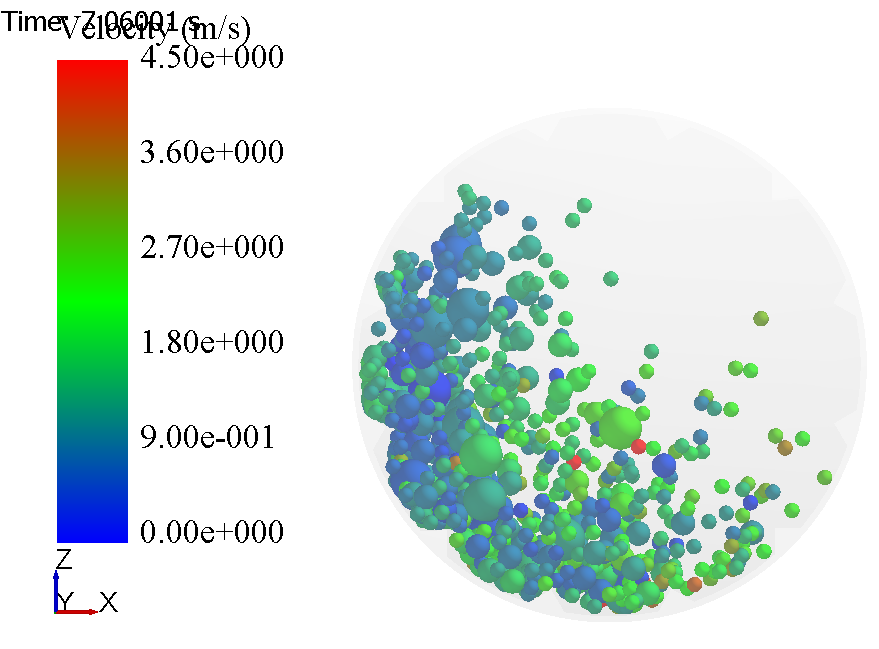
\includegraphics[width=\textwidth]{Images/Resultados/Sim1/sim1.PNG}
		\caption{Perfil de velocidades durante la molienda.}
	\end{subfigure}
	\hfill
	\begin{subfigure}[b]{0.94\textwidth}
		\centering
		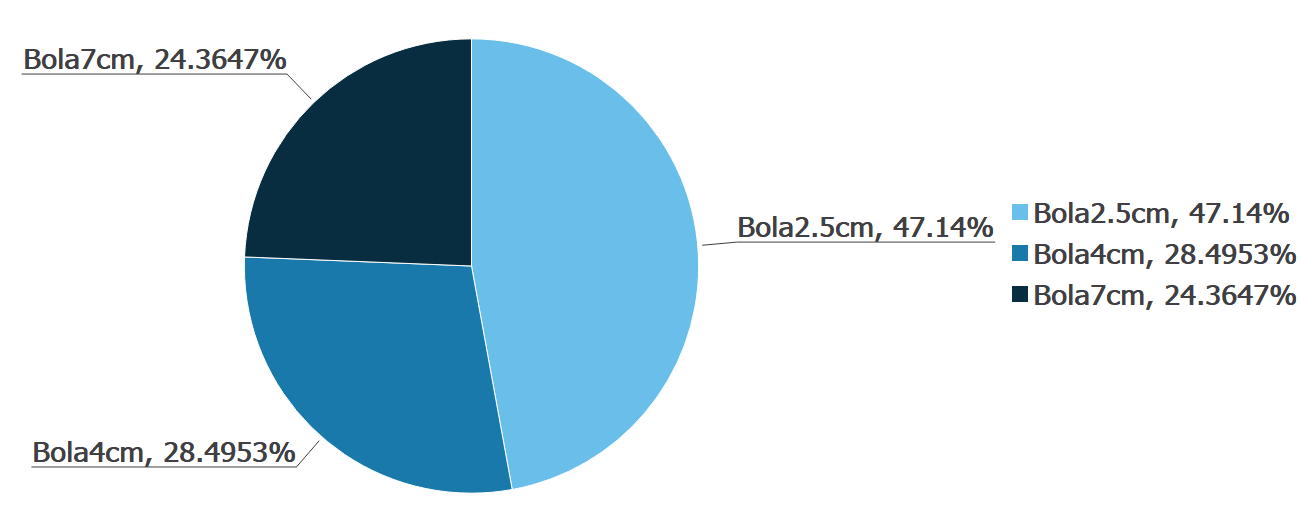
\includegraphics[width=\textwidth]{Images/Resultados/Sim1/dist1.PNG}
	\caption{Distribuci\'on de la energ\'ia de impacto por tipo de bola.}
	\end{subfigure}
	\caption{Resultados iniciales de la primera iteraci\'on.}
	\label{resul1}
\end{figure}


\noindent
\justify

De la Figura \ref{resul1}, se puede apreciar que las esferas de menor di\'ametro $\left( 2.5 [cm] \right)$ tienden a alcanzar velocidades de hasta $4.5 \left[m/s^2 \right]$ de magnitud. La distribuci\'on de la energ\'ia de impacto tiende a ser mayor, para esta configuraci\'on, por parte de las bolas de menor tama\~no con un $47.1 \%$, seguido por las bolas de $4 [cm]$ con un porcentaje del $28.5 \%$ y, finalmente, las bolas de $7 [cm]$, que presentan una distribuci\'on del $24.4 \%$ de la energ\'ia de impacto transmitida.

\begin{figure}[h!]
\centering
\begin{tikzpicture}
	\begin{axis}[grid = both, minor tick num=2,
			title = \textbf{Tiempo vs Energ\'ia cin\'etica},
			xlabel = {Tiempo $[s]$},
			ylabel = {Energ\'ia cin\'etica $[J]$},
			width=\textwidth]
	\addplot[smooth, mark=*, blue!60!black] table [x=TIME, y=E2.5] {Results/res1.txt};
	\addlegendentry{Bolas $2.5 [cm]$}
	\addplot table [x=TIME, y=E4] {Results/res1.txt};
	\addlegendentry{Bolas $4 [cm]$}
	\addplot[smooth, mark=*, green!70!red] table [x=TIME, y=E7] {Results/res1.txt};
	\addlegendentry{Bolas $7 [cm]$}
	\end{axis}
\end{tikzpicture}
\caption{Valor de la energ\'ia cin\'etica m\'axima, por tipo de bola, en el tiempo.}
\label{res1}
\end{figure}

\noindent
\justify

En la Figura \ref{res1}, se observa el valor de la energ\'ia cin\'etica m\'axima, antes de la colisi\'on, d\'onde se observa que la energ\'ia transmitida por las esferas de $7 [cm]$ tiende a ser cerca del doble de las transmitidas por las de $2.5 [cm]$; y que la energ\'ia cin\'etica de las bolas de $2.5 [cm]$ y las de $4 [cm]$ no presenta una diferencia considerable (cerca de $0.5 [J]$ de diferencia).

\noindent
\justify

La etapa de \textit{movimiento parab\'olico} de las bolas dur\'o, en promedio, $0.41 [s]$; arrojando un \textbf{error de simulaci\'on} del $4.65 \%$ (compar\'andolo con el valor de $0.43 [s]$ calculado en la secci\'on \ref{cinema}).

\noindent
\justify

Con base a los resultados mostrados en las Figuras \ref{resul1} y \ref{res1}, se observa que las bolas de $4 [cm]$ no representan un \textit{aporte considerable} en el desempe\~no del molino, por lo que se cambiar\'an por esferas de $5 [cm]$ en futuros an\'alisis.  

\subsection{Segunda iteraci\'on} \label{segunda}

\noindent
\justify

Con base en los resultados obtenidos en la secci\'on \ref{primera}, se realiz\'o una simulaci\'on con los siguientes datos: 10 aletas de $h = 10 [mm]$ y $\theta = 45 [\degree ]$; bolas de $2.5 [cm]$, $5 [cm]$ y $7 [cm]$. Obteniendo los resultados mostrados a continuaci\'on.

\begin{figure}[h!]
	\centering
	\begin{subfigure}[b]{0.66\textwidth}
		\centering
		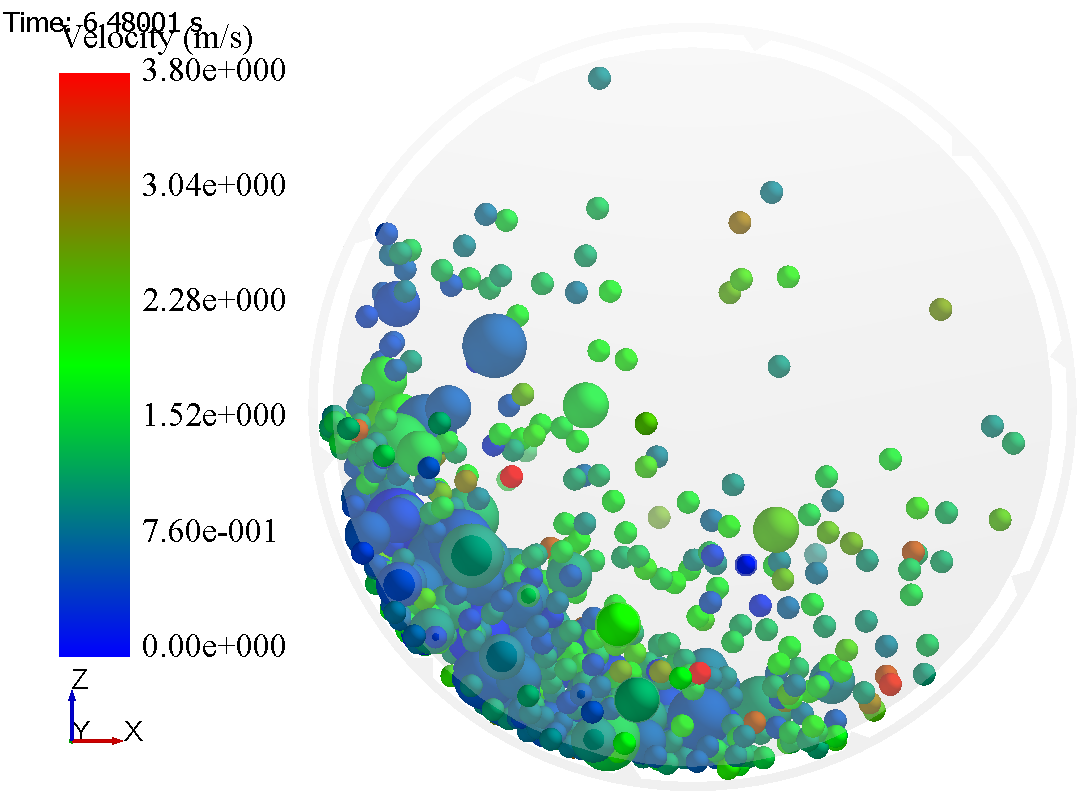
\includegraphics[width=\textwidth]{Images/Resultados/Sim2/sim2.PNG}
		\caption{Perfil de velocidades durante la molienda.}
	\end{subfigure}
	\hfill
	\begin{subfigure}[b]{0.9\textwidth}
		\centering
		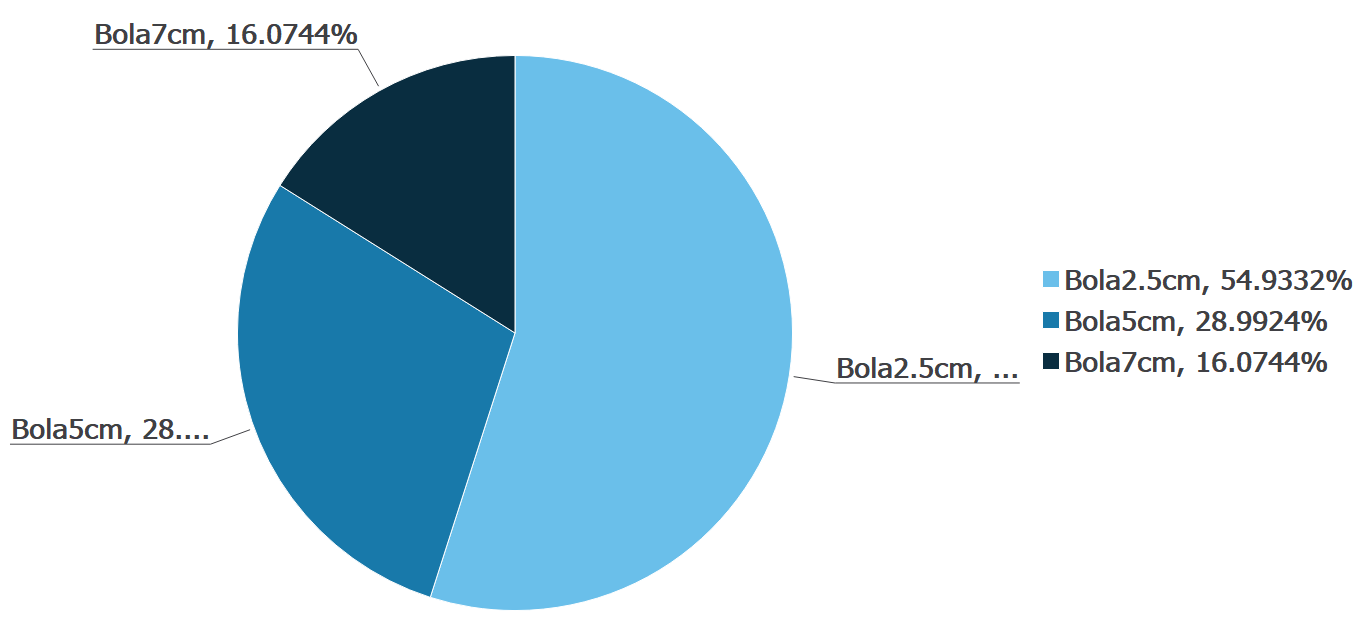
\includegraphics[width=\textwidth]{Images/Resultados/Sim2/dist2.PNG}
	\caption{Distribuci\'on de la energ\'ia de impacto por tipo de bola.}
	\end{subfigure}
	\caption{Resultados iniciales de la segunda iteraci\'on.}
	\label{resul2}
\end{figure}

\noindent
\justify

De la Figura \ref{resul2}, se puede apreciar que las esferas de menor di\'ametro $\left( 2.5 [cm] \right)$ tienden a alcanzar velocidades de hasta $3.8 \left[m/s^2 \right]$ de magnitud. La distribuci\'on de la energ\'ia de impacto tiende a ser mayor, para esta configuraci\'on, por parte de las bolas de menor tama\~no con un $54.93 \%$, seguido por las bolas de $5 [cm]$ con un porcentaje del $28.99 \%$ y, finalmente, las bolas de $7 [cm]$, que presentan una distribuci\'on del $16.07 \%$ de la energ\'ia de impacto transmitida.

\begin{figure}[h!]
\centering
\begin{tikzpicture}
	\begin{axis}[grid = both, minor tick num=2,
			title = \textbf{Tiempo vs Energ\'ia cin\'etica},
			xlabel = {Tiempo $[s]$},
			ylabel = {Energ\'ia cin\'etica $[J]$},
			width=\textwidth]
	\addplot[smooth, mark=*, blue!60!black] table [x=TIME, y=E2.5] {Results/res2.txt};
	\addlegendentry{Bolas $2.5 [cm]$}
	\addplot table [x=TIME, y=E5] {Results/res2.txt};
	\addlegendentry{Bolas $5 [cm]$}
	\addplot[smooth, mark=*, green!70!red] table [x=TIME, y=E7] {Results/res2.txt};
	\addlegendentry{Bolas $7 [cm]$}
	\end{axis}
\end{tikzpicture}
\caption{Valor de la energ\'ia cin\'etica m\'axima, por tipo de bola, en el tiempo.}
\label{res2}
\end{figure}

\noindent
\justify

Al igual que en la Figura \ref{res1}, en la Figura \ref{res2} se observa el valor de la energ\'ia cin\'etica m\'axima antes de la colisi\'on, d\'onde se detalla que la energ\'ia transmitida por las esferas de $7 [cm]$ tiende a ser m\'as del doble de las transmitidas por las de $2.5 [cm]$. A diferencia de la Figura \ref{res1}, la distribuci\'on de la energ\'ia de impacto por tipo de bola es m\'as clara, presentando diferencias apreciables entre s\'i, de m\'as del $50 \%$. Sin embargo, los valores m\'aximos de energ\'ia son significativamente inferiores con esta configuraci\'on; lo que permite concluir que las bolas de $5 [cm]$ confieren mayor eficiencia a la molienda, pero se reduce la efectividad debido a la geometr\'ia de las aletas.

\noindent
\justify

La etapa de \textit{movimiento parab\'olico} de las bolas dur\'o, en promedio, $0.39 [s]$; arrojando un \textbf{error de simulaci\'on} del $9.3 \%$ (compar\'andolo con el valor de $0.43 [s]$ calculado en la secci\'on \ref{cinema}).

\subsection{Tercera iteraci\'on}

\noindent
\justify

Con base en los resultados obtenidos en la secci\'on \ref{segunda}, se desarroll\'o una simulaci\'on con los siguientes par\'ametros: 10 aletas de $h = 40 [mm]$ y $\theta = 30 [\degree ]$; bolas de $7 [cm]$, $5 [cm]$ y $2.5 [cm]$.

\begin{figure}[h!]
	\centering
	\begin{subfigure}[b]{0.66\textwidth}
		\centering
		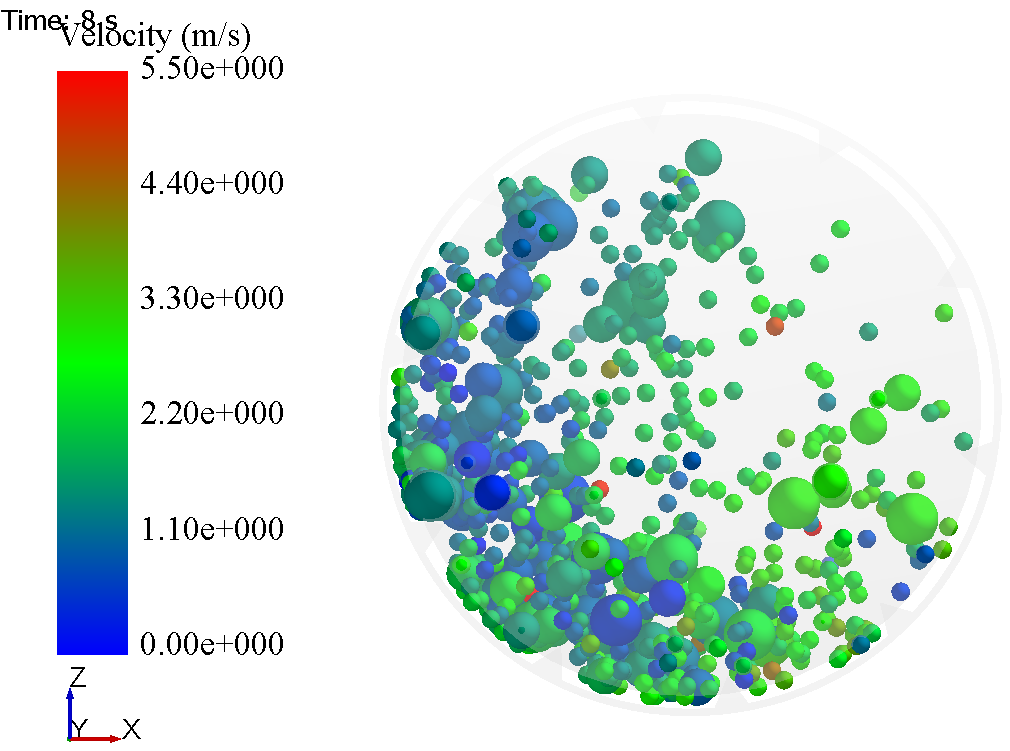
\includegraphics[width=\textwidth]{Images/Resultados/Sim3/sim3.PNG}
		\caption{Perfil de velocidades durante la molienda.}
	\end{subfigure}
	\hfill
	\begin{subfigure}[b]{0.9\textwidth}
		\centering
		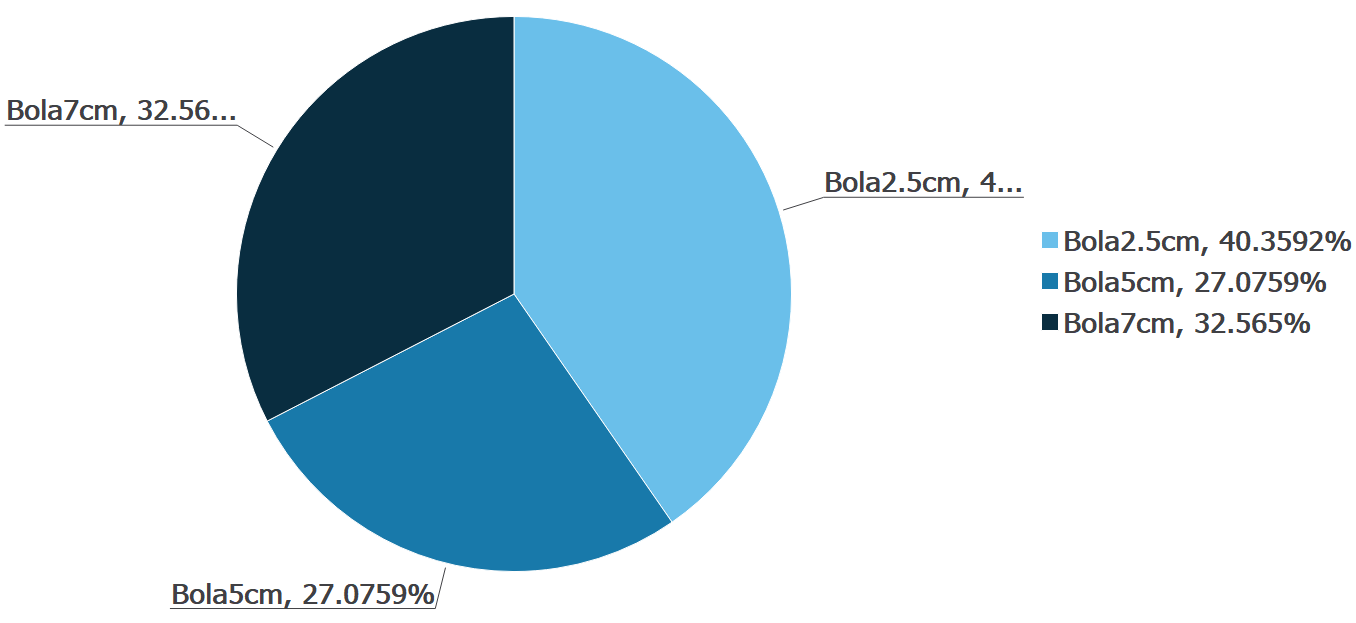
\includegraphics[width=\textwidth]{Images/Resultados/Sim3/dist3.PNG}
	\caption{Distribuci\'on de la energ\'ia de impacto por tipo de bola.}
	\end{subfigure}
	\caption{Resultados iniciales de la tercera iteraci\'on.}
	\label{resul3}
\end{figure}

\noindent
\justify

En la Figura \ref{resul3}, se puede apreciar que las esferas de $2.5 [cm]$ contin\'uan alcanzando las mayores velocidades, llegando con esta configuraci\'on hasta los $5.5 \left[m/s^2 \right]$ de magnitud. La distribuci\'on de la energ\'ia de impacto tiende a ser m\'as equitativa que en las iteraciones anteriores, donde las bolas de menor tama\~no presentan un $40.35 \%$ de distribuci\'on, seguido por las bolas de $7 [cm]$ con un porcentaje del $32.56 \%$ y, finalmente, las bolas de $5 [cm]$, que presentan una distribuci\'on del $27.08 \%$ de la energ\'ia de impacto transmitida.


\begin{figure}[h!]
\centering
\begin{tikzpicture}
	\begin{axis}[grid = both, minor tick num=2,
			title = \textbf{Tiempo vs Energ\'ia cin\'etica},
			xlabel = {Tiempo $[s]$},
			ylabel = {Energ\'ia cin\'etica $[J]$},
			width=\textwidth]
	\addplot[smooth, mark=*, blue!60!black] table [x=TIME, y=E2.5] {Results/res3.txt};
	\addlegendentry{Bolas $2.5 [cm]$}
	\addplot table [x=TIME, y=E5] {Results/res3.txt};
	\addlegendentry{Bolas $5 [cm]$}
	\addplot[smooth, mark=*, green!70!red] table [x=TIME, y=E7] {Results/res3.txt};
	\addlegendentry{Bolas $7 [cm]$}
	\end{axis}
\end{tikzpicture}
\caption{Valor de la energ\'ia cin\'etica m\'axima, por tipo de bola, en el tiempo.}
\label{res3}
\end{figure}

\noindent
\justify

En la Figura \ref{res3}, se aprecia el valor de la energ\'ia cin\'etica m\'axima antes de la colisi\'on. Compar\'andola con los resultados anteriores, se observa una mayor energ\'ia de impacto y una mejor distribuci\'on entre los diferentes tipos de bola, lo que hace de esta alternativa, no s\'olo la m\'as eficiente, sino tambi\'en la m\'as efectiva.


\newpage

\begin{center}
	\section{Resultado}
\end{center}

\noindent
\justify

Conociendo la distribuci\'on geom\'etrica de las aletas que mejor distribuci\'on de energ\'ia y mayor magnitud de energ\'ia de impacto por tipo de bola produce, se desarroll\'o una nueva simulaci\'on num\'erica con el material a pulverizar (agente dispersante y material vegetal) para detallar la forma en c\'omo se distribuye el material durante la etapa de molienda. La proporci\'on de llenado, en t\'erminos volum\'etricos, es la siguiente: $20\%$ lo ocupan las bolas del molino, $16\%$ el material vegetal y el $14\%$ el agente dispersante.

\begin{figure}[h!]
	\centering
	\begin{subfigure}[b]{0.6\textwidth}
		\centering
		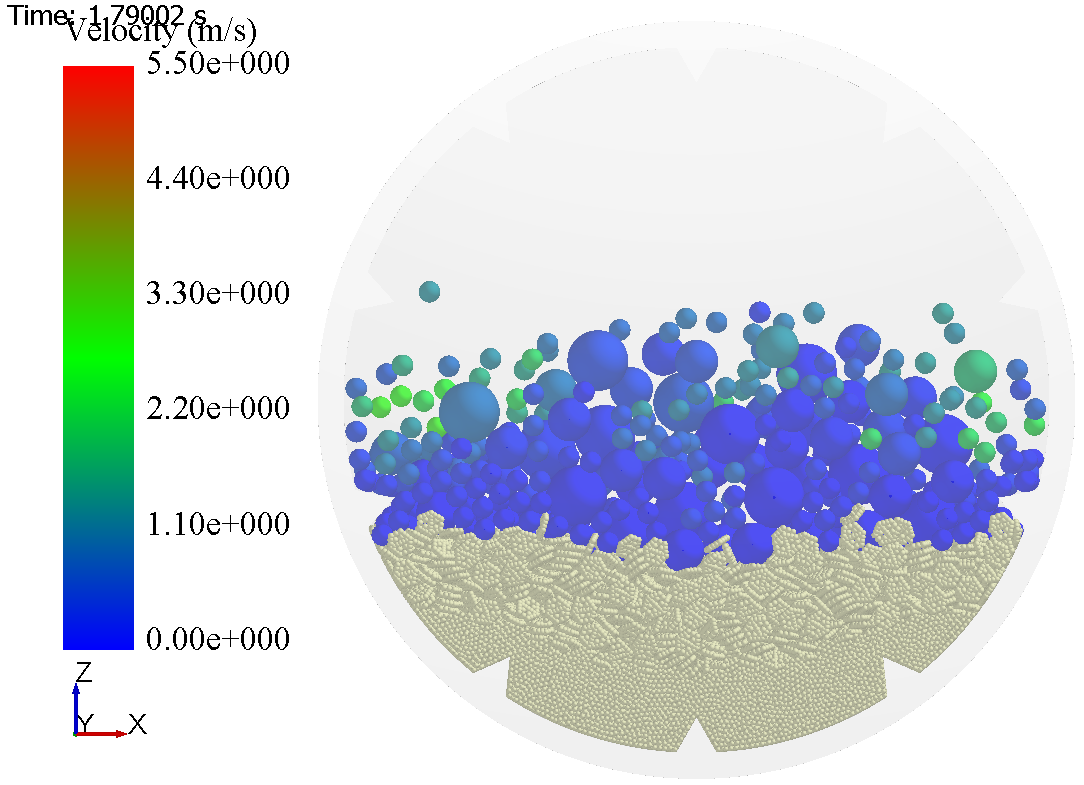
\includegraphics[width=\textwidth]{Images/Resultados/Real.PNG}
		\caption{Material a moler.}
	\end{subfigure}
	\hfill
	\begin{subfigure}[b]{0.6\textwidth}
		\centering
		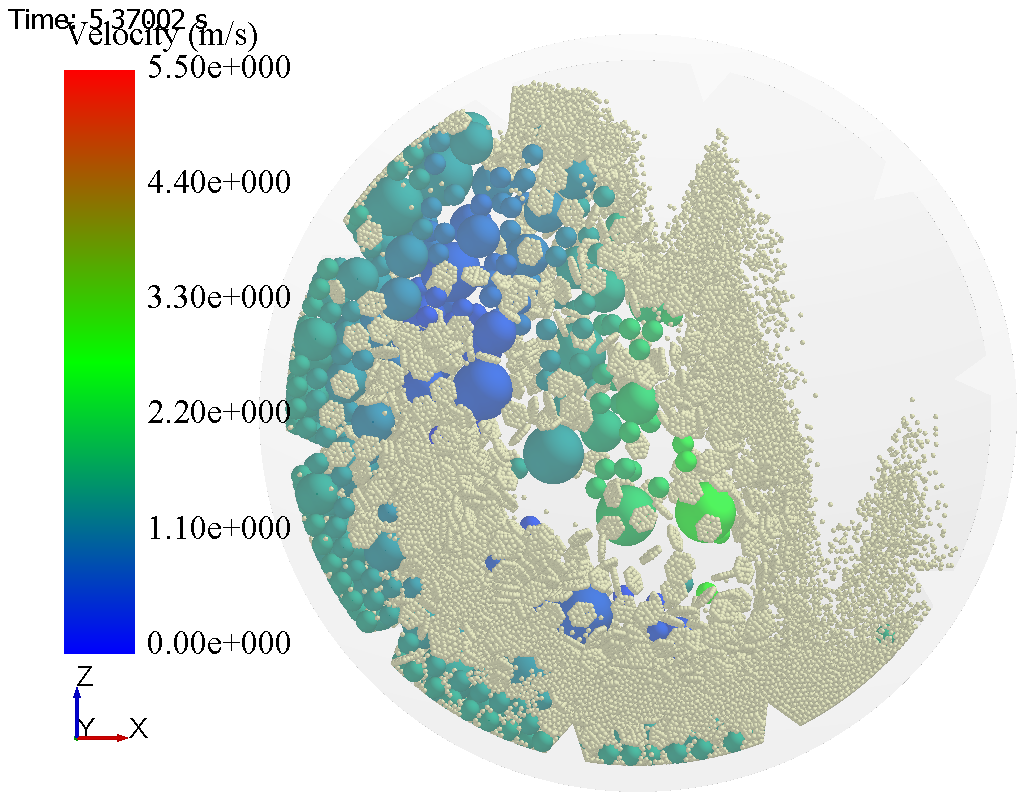
\includegraphics[width=\textwidth]{Images/Resultados/total.PNG}
	\caption{Molienda.}
	\end{subfigure}
	\caption{Simulaci\'on con el material a pulverizar.}
	\label{resul4}
\end{figure}



\newpage

\begin{center}
	\section{An\'alisis de resultados y conclusiones}
\end{center}

\noindent
\justify

De las iteraciones desarrolladas, la configuraci\'on de aletas que mejor desempe\~no obtuvo fue la tercera (10 aletas de $h=40 [mm]$, $\theta = 30 [\degree ]$ y bolas de: $7[cm]$, $5[cm]$ y $2.5[cm]$; como se observa en la Figura \ref{sol}), debido a que obtuvo la mayor energ\'ia cin\'etica media y la distribuci\'on de energ\'ia de impacto m\'as equitativa durante la etapa de molienda. Como se observa en la Figura \ref{resul4}, este sistema cumple el objetivo requerido por la planta de extracci\'on debido a que las esferas de $7 [cm]$ y $5 [cm]$ presentan la energ\'ia suficiente para disminuir el tama\~no de part\'icula de tallos y ramas, mientras que las bolas de $2.5 [cm]$ lograr\'an pulverizar el material por debajo de los $250 [\mu m]$.

\begin{figure}[h!]
\centering
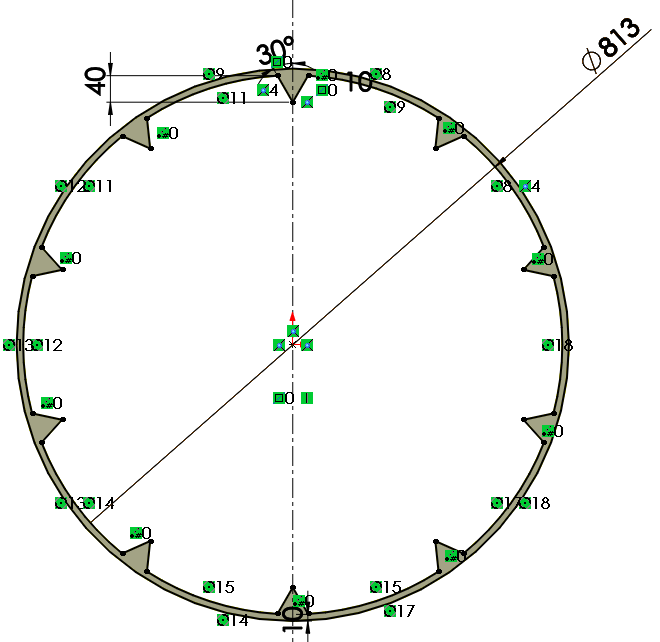
\includegraphics[width=\textwidth]{Images/Resultados/res.PNG}
\caption{Dise\~no funcional del molino.}
\label{sol}
\end{figure}
\bibliography{library}
\end{document}

